\chapter{Experiment}
In this section we explain our experimentation with multi-task learning for relation classification. We begin by describing related work on deep multi-task learning for natural language processing tasks and relation extraction. Our focus is to investigate the impact of multi-task learning on generalization error on a target task introduced in the first section. We continue by describing each auxiliary task. Finally, we describe the neural network architecture and algorithm used for generating empirical data.
\section{Related Work}
To our knowledge, there hasn't been any experimental work done on deep multi-task learning for relation classification despite the popularity of these techniques in natural language processing in general. The work of \citet{jiang2009} is perhaps most closely related to our own. She demonstrates a technique for sharing weights between logistic regression classifiers trained for binary classification of a target relation and auxiliary relation when there is only a small number of seed training instances available for the target task. 

The input to these binary classifiers are engineered linguistic features based on syntactic and dependency parse trees. She finds that sharing components of the weight vectors for each of these classifiers improves the F1 score on a validation set compared to learning the weight vectors in a single-task fashion.

Moreover, she finds that the benefit of weight sharing decreases as the number of seed instances is increased. In particular, she finds that when the number of target examples exceed a 1000 samples single task learning produces better results than multi-task learning.
\\\\
\citet{collobert2011} is one of the earliest works that detail how to solve natural language processing tasks with neural networks. They focus on neural networks for sequence prediction problems. Specifically, they use two different neural network architectures for predicting tags for words by considering a window of neighboring words around the target word, transform this window into a matrix of concatenated word-vectors and feed this into a neural network. The major contribution of this technique was to show that state-of-the-art performance was possible for these tagging tasks without manual feature engineering, but simply by learning word vectors and convolutional filters directly from the words.

\citet{collobert2011} also experimented with deep multi-task learning through hard weight sharing and found that weight sharing in general increased performance on most of the tasks they considered.
\\\\
\citet{bingel2017} performs a thorough experiment on deep multi-task learning using recurrent neural networks for sequence prediction problems in natural language processing. They run experiments of 90 different configurations of target and auxiliary task and compare generalization error for the target task when compared to single-task learning. Their goal is to investigate correlation between dataset statistics and characteristics in single-task learning that are good predictors for gains in multi-task learning.

They find that the best predictor for multi-task learning gains is single-task learning curves over gradient descent iterations. Specifically, if the target task generalization error quickly plateaus, learning it simultaneously with an auxiliary task that doesn't plateau is likely to improve generalization. They speculate this happens because the inclusion of an auxiliary task can move neural network weights out of local minima during training.
\\\\
Neural networks have also been tested for sentence classification problems such as relation classification. \citet{kim2014} design a convolutional neural network for sentence classification and tests it on a number of sentence classification tasks such as sentiment analysis and semantic category prediction in a single-task learning setting. His architecture achieves state-of-the-art performance on a number of these tasks without any manual feature engineering.

\citet{nguyen2015} and adapts the work of \citet{kim2014} to the relation classification problem. Their addition to the architecture is a mechanism for marking the relation arguments in the input. This leads to state-of-the-art performance. They do not consider multi-task learning.
\\\\
\citet{zhang2015} investigate the performance of recurrent neural networks on the relation extraction problem. They suggest a simple bi-directional recurrent architecture where the relation arguments are marked simply by special tokens that indicate the beginning and end of each argument. With this architecture they achieve almost state-of-the-art results close to the results of \citet{nguyen2015}. They find that for sentences where the relation arguments are far apart, the recurrent architecture outperforms the convolutional architecture.
\section{Target Task}
\label{target_task}
We have chosen a target relation classification dataset which will act as a benchmark across our experiments in order to empirically investigate the dynamics of sample complexity for multi-task relation classification. The SemEval 2010 Task 8 dataset has arguably become somewhat of a standard for relation classification papers, and so is a reasonable choice for the role of target task in this context \citep{hendrickx2009}.
\\\\
The SemEval 2010 Task 8 dataset consists of 10,717 English sentences. Each sentence is annotated with exactly one of the following semantic relations:

\begin{description}[labelindent=4em,leftmargin=4em]
	\item [Cause-Effect] An event or object leads to an
effect. Example: \emph{those [cancers] were caused
by radiation [exposures].}
	\item [Instrument-Agency] An agent uses an instrument. Example: \emph{[phone] [operator].}
	\item [Product-Producer] A producer causes a product to exist. Example: \emph{a [factory] manufactures [suits].}
	\item [Content-Container] An object is physically stored in a delineated area of space. Example: \emph{a [bottle] full of [honey] was weighed}
	\item [Entity-Origin] An entity is coming or is derived from an origin (e.g., position or material). Example: \emph{[letters] from foreign [countries].}
	\item [Entity-Destination] An entity is moving towards a destination. Example: \emph{the [boy] went to [bed].}
	\item [Component-Whole] An object is a component of a larger whole. Example: \emph{my [apartment] has a large [kitchen].}
	\item [Member-Collection] A member forms a nonfunctional part of a collection. Example: \emph{there are many [trees] in the [forest].}
	\item [Message-Topic] A message, written or spoken, is about a topic. Example: \emph{the [lecture] was about [semantics].}
	\item [Other] Any other relation.
\end{description}
\noindent
SemEval 2010 Task 8 is not a traditional relation classification task. In particular, the objective of traditional relation extraction is to identify semantic relationships between named entities. In the SemEval dataset however, the annotated relationships are between head words of nominal phrases, for example \textit{Message-Topic(lecture, semantics)} in the sentence \textit{the lecture was about semantics} where neither \textit{lecture} nor \textit{semantics} are named entities.
\\\\
Moreover, the annotation process for the SemEval dataset includes some restrictions which are designed to make the resulting learning problem easier. Firstly, the annotators exclude sentences where relationships depend on discourse knowledge, for example when one of the arguments are pronouns. Secondly, sentences where the relation arguments occur in different sentential clauses are excluded. For example, we could argue that the relationship \textit{Instrument-Agency(man, unicycle)} exists in the sentence \textit{the man, who rides a unicycle, came to see me.}, but since the arguments occur in different sentential clauses it would be excluded from the SemEval dataset.
\\\\
The annotators aimed for a uniform distribution of relations in the SemEval dataset. To this end, they initially collected approximately 1200 sentences for each relation category by pattern based web search. This ultimately lead to the distribution shown in figure \ref{semeval_dist}. One consequence of this selection procedure is that the label distribution does not follow the distribution of relations found in natural language data in the wild.
\\\\
Ideally, we'd like to be able to make conclusions about the usefulness of multi-task learning for relation classification in general and not just on SemEval 2010 Task 8 based on the results in this thesis. This is possible to the extent that the SemEval data is a realistic sample and that the target relations are general enough that they are useful for a wide range of domains. As discussed above, both of these qualities can be called into question.
\\\\
\citet{handschuh2016} provides a brief discussion of the generality of SemEval 2010 Task 8. In addition to the limitations we have already pointed out, they highlight that the relations in the SemEval dataset are mainly concerned with relations between concrete, physical objects. Taken together, the limitations of SemEval 2010 Task 8 could indicate that a need exists for authoring a more general relation classification task that is more appropriate as a benchmark. At this time however, we use the SemEval dataset as target task in our experiments because of its prevalence in the research literature, despite these points of criticism.

\begin{figure}
	\center
	%% Creator: Matplotlib, PGF backend
%%
%% To include the figure in your LaTeX document, write
%%   \input{<filename>.pgf}
%%
%% Make sure the required packages are loaded in your preamble
%%   \usepackage{pgf}
%%
%% Figures using additional raster images can only be included by \input if
%% they are in the same directory as the main LaTeX file. For loading figures
%% from other directories you can use the `import` package
%%   \usepackage{import}
%% and then include the figures with
%%   \import{<path to file>}{<filename>.pgf}
%%
%% Matplotlib used the following preamble
%%   \usepackage{fontspec}
%%   \setmainfont{Palatino}
%%   \setsansfont{Lucida Grande}
%%   \setmonofont{Andale Mono}
%%
\begingroup%
\makeatletter%
\begin{pgfpicture}%
\pgfpathrectangle{\pgfpointorigin}{\pgfqpoint{4.849939in}{3.853687in}}%
\pgfusepath{use as bounding box, clip}%
\begin{pgfscope}%
\pgfsetbuttcap%
\pgfsetmiterjoin%
\definecolor{currentfill}{rgb}{1.000000,1.000000,1.000000}%
\pgfsetfillcolor{currentfill}%
\pgfsetlinewidth{0.000000pt}%
\definecolor{currentstroke}{rgb}{1.000000,1.000000,1.000000}%
\pgfsetstrokecolor{currentstroke}%
\pgfsetdash{}{0pt}%
\pgfpathmoveto{\pgfqpoint{0.000000in}{0.000000in}}%
\pgfpathlineto{\pgfqpoint{4.849939in}{0.000000in}}%
\pgfpathlineto{\pgfqpoint{4.849939in}{3.853687in}}%
\pgfpathlineto{\pgfqpoint{0.000000in}{3.853687in}}%
\pgfpathclose%
\pgfusepath{fill}%
\end{pgfscope}%
\begin{pgfscope}%
\pgfsetbuttcap%
\pgfsetmiterjoin%
\definecolor{currentfill}{rgb}{1.000000,1.000000,1.000000}%
\pgfsetfillcolor{currentfill}%
\pgfsetlinewidth{0.000000pt}%
\definecolor{currentstroke}{rgb}{0.000000,0.000000,0.000000}%
\pgfsetstrokecolor{currentstroke}%
\pgfsetstrokeopacity{0.000000}%
\pgfsetdash{}{0pt}%
\pgfpathmoveto{\pgfqpoint{0.347222in}{1.059136in}}%
\pgfpathlineto{\pgfqpoint{4.832439in}{1.059136in}}%
\pgfpathlineto{\pgfqpoint{4.832439in}{3.813269in}}%
\pgfpathlineto{\pgfqpoint{0.347222in}{3.813269in}}%
\pgfpathclose%
\pgfusepath{fill}%
\end{pgfscope}%
\begin{pgfscope}%
\pgfpathrectangle{\pgfqpoint{0.347222in}{1.059136in}}{\pgfqpoint{4.485217in}{2.754132in}} %
\pgfusepath{clip}%
\pgfsetbuttcap%
\pgfsetmiterjoin%
\definecolor{currentfill}{rgb}{0.121569,0.466667,0.705882}%
\pgfsetfillcolor{currentfill}%
\pgfsetlinewidth{0.000000pt}%
\definecolor{currentstroke}{rgb}{0.000000,0.000000,0.000000}%
\pgfsetstrokecolor{currentstroke}%
\pgfsetstrokeopacity{0.000000}%
\pgfsetdash{}{0pt}%
\pgfpathmoveto{\pgfqpoint{0.551096in}{1.059136in}}%
\pgfpathlineto{\pgfqpoint{0.883950in}{1.059136in}}%
\pgfpathlineto{\pgfqpoint{0.883950in}{2.766698in}}%
\pgfpathlineto{\pgfqpoint{0.551096in}{2.766698in}}%
\pgfpathclose%
\pgfusepath{fill}%
\end{pgfscope}%
\begin{pgfscope}%
\pgfpathrectangle{\pgfqpoint{0.347222in}{1.059136in}}{\pgfqpoint{4.485217in}{2.754132in}} %
\pgfusepath{clip}%
\pgfsetbuttcap%
\pgfsetmiterjoin%
\definecolor{currentfill}{rgb}{0.121569,0.466667,0.705882}%
\pgfsetfillcolor{currentfill}%
\pgfsetlinewidth{0.000000pt}%
\definecolor{currentstroke}{rgb}{0.000000,0.000000,0.000000}%
\pgfsetstrokecolor{currentstroke}%
\pgfsetstrokeopacity{0.000000}%
\pgfsetdash{}{0pt}%
\pgfpathmoveto{\pgfqpoint{0.967164in}{1.059136in}}%
\pgfpathlineto{\pgfqpoint{1.300019in}{1.059136in}}%
\pgfpathlineto{\pgfqpoint{1.300019in}{2.670304in}}%
\pgfpathlineto{\pgfqpoint{0.967164in}{2.670304in}}%
\pgfpathclose%
\pgfusepath{fill}%
\end{pgfscope}%
\begin{pgfscope}%
\pgfpathrectangle{\pgfqpoint{0.347222in}{1.059136in}}{\pgfqpoint{4.485217in}{2.754132in}} %
\pgfusepath{clip}%
\pgfsetbuttcap%
\pgfsetmiterjoin%
\definecolor{currentfill}{rgb}{0.121569,0.466667,0.705882}%
\pgfsetfillcolor{currentfill}%
\pgfsetlinewidth{0.000000pt}%
\definecolor{currentstroke}{rgb}{0.000000,0.000000,0.000000}%
\pgfsetstrokecolor{currentstroke}%
\pgfsetstrokeopacity{0.000000}%
\pgfsetdash{}{0pt}%
\pgfpathmoveto{\pgfqpoint{1.383232in}{1.059136in}}%
\pgfpathlineto{\pgfqpoint{1.716087in}{1.059136in}}%
\pgfpathlineto{\pgfqpoint{1.716087in}{2.518826in}}%
\pgfpathlineto{\pgfqpoint{1.383232in}{2.518826in}}%
\pgfpathclose%
\pgfusepath{fill}%
\end{pgfscope}%
\begin{pgfscope}%
\pgfpathrectangle{\pgfqpoint{0.347222in}{1.059136in}}{\pgfqpoint{4.485217in}{2.754132in}} %
\pgfusepath{clip}%
\pgfsetbuttcap%
\pgfsetmiterjoin%
\definecolor{currentfill}{rgb}{0.121569,0.466667,0.705882}%
\pgfsetfillcolor{currentfill}%
\pgfsetlinewidth{0.000000pt}%
\definecolor{currentstroke}{rgb}{0.000000,0.000000,0.000000}%
\pgfsetstrokecolor{currentstroke}%
\pgfsetstrokeopacity{0.000000}%
\pgfsetdash{}{0pt}%
\pgfpathmoveto{\pgfqpoint{1.799301in}{1.059136in}}%
\pgfpathlineto{\pgfqpoint{2.132155in}{1.059136in}}%
\pgfpathlineto{\pgfqpoint{2.132155in}{2.312266in}}%
\pgfpathlineto{\pgfqpoint{1.799301in}{2.312266in}}%
\pgfpathclose%
\pgfusepath{fill}%
\end{pgfscope}%
\begin{pgfscope}%
\pgfpathrectangle{\pgfqpoint{0.347222in}{1.059136in}}{\pgfqpoint{4.485217in}{2.754132in}} %
\pgfusepath{clip}%
\pgfsetbuttcap%
\pgfsetmiterjoin%
\definecolor{currentfill}{rgb}{0.121569,0.466667,0.705882}%
\pgfsetfillcolor{currentfill}%
\pgfsetlinewidth{0.000000pt}%
\definecolor{currentstroke}{rgb}{0.000000,0.000000,0.000000}%
\pgfsetstrokecolor{currentstroke}%
\pgfsetstrokeopacity{0.000000}%
\pgfsetdash{}{0pt}%
\pgfpathmoveto{\pgfqpoint{2.215369in}{1.059136in}}%
\pgfpathlineto{\pgfqpoint{2.548224in}{1.059136in}}%
\pgfpathlineto{\pgfqpoint{2.548224in}{2.270954in}}%
\pgfpathlineto{\pgfqpoint{2.215369in}{2.270954in}}%
\pgfpathclose%
\pgfusepath{fill}%
\end{pgfscope}%
\begin{pgfscope}%
\pgfpathrectangle{\pgfqpoint{0.347222in}{1.059136in}}{\pgfqpoint{4.485217in}{2.754132in}} %
\pgfusepath{clip}%
\pgfsetbuttcap%
\pgfsetmiterjoin%
\definecolor{currentfill}{rgb}{0.121569,0.466667,0.705882}%
\pgfsetfillcolor{currentfill}%
\pgfsetlinewidth{0.000000pt}%
\definecolor{currentstroke}{rgb}{0.000000,0.000000,0.000000}%
\pgfsetstrokecolor{currentstroke}%
\pgfsetstrokeopacity{0.000000}%
\pgfsetdash{}{0pt}%
\pgfpathmoveto{\pgfqpoint{2.631437in}{1.059136in}}%
\pgfpathlineto{\pgfqpoint{2.964292in}{1.059136in}}%
\pgfpathlineto{\pgfqpoint{2.964292in}{2.243413in}}%
\pgfpathlineto{\pgfqpoint{2.631437in}{2.243413in}}%
\pgfpathclose%
\pgfusepath{fill}%
\end{pgfscope}%
\begin{pgfscope}%
\pgfpathrectangle{\pgfqpoint{0.347222in}{1.059136in}}{\pgfqpoint{4.485217in}{2.754132in}} %
\pgfusepath{clip}%
\pgfsetbuttcap%
\pgfsetmiterjoin%
\definecolor{currentfill}{rgb}{0.121569,0.466667,0.705882}%
\pgfsetfillcolor{currentfill}%
\pgfsetlinewidth{0.000000pt}%
\definecolor{currentstroke}{rgb}{0.000000,0.000000,0.000000}%
\pgfsetstrokecolor{currentstroke}%
\pgfsetstrokeopacity{0.000000}%
\pgfsetdash{}{0pt}%
\pgfpathmoveto{\pgfqpoint{3.047506in}{1.059136in}}%
\pgfpathlineto{\pgfqpoint{3.380360in}{1.059136in}}%
\pgfpathlineto{\pgfqpoint{3.380360in}{2.215872in}}%
\pgfpathlineto{\pgfqpoint{3.047506in}{2.215872in}}%
\pgfpathclose%
\pgfusepath{fill}%
\end{pgfscope}%
\begin{pgfscope}%
\pgfpathrectangle{\pgfqpoint{0.347222in}{1.059136in}}{\pgfqpoint{4.485217in}{2.754132in}} %
\pgfusepath{clip}%
\pgfsetbuttcap%
\pgfsetmiterjoin%
\definecolor{currentfill}{rgb}{0.121569,0.466667,0.705882}%
\pgfsetfillcolor{currentfill}%
\pgfsetlinewidth{0.000000pt}%
\definecolor{currentstroke}{rgb}{0.000000,0.000000,0.000000}%
\pgfsetstrokecolor{currentstroke}%
\pgfsetstrokeopacity{0.000000}%
\pgfsetdash{}{0pt}%
\pgfpathmoveto{\pgfqpoint{3.463574in}{1.059136in}}%
\pgfpathlineto{\pgfqpoint{3.796429in}{1.059136in}}%
\pgfpathlineto{\pgfqpoint{3.796429in}{1.995541in}}%
\pgfpathlineto{\pgfqpoint{3.463574in}{1.995541in}}%
\pgfpathclose%
\pgfusepath{fill}%
\end{pgfscope}%
\begin{pgfscope}%
\pgfpathrectangle{\pgfqpoint{0.347222in}{1.059136in}}{\pgfqpoint{4.485217in}{2.754132in}} %
\pgfusepath{clip}%
\pgfsetbuttcap%
\pgfsetmiterjoin%
\definecolor{currentfill}{rgb}{0.121569,0.466667,0.705882}%
\pgfsetfillcolor{currentfill}%
\pgfsetlinewidth{0.000000pt}%
\definecolor{currentstroke}{rgb}{0.000000,0.000000,0.000000}%
\pgfsetstrokecolor{currentstroke}%
\pgfsetstrokeopacity{0.000000}%
\pgfsetdash{}{0pt}%
\pgfpathmoveto{\pgfqpoint{3.879642in}{1.059136in}}%
\pgfpathlineto{\pgfqpoint{4.212497in}{1.059136in}}%
\pgfpathlineto{\pgfqpoint{4.212497in}{1.912917in}}%
\pgfpathlineto{\pgfqpoint{3.879642in}{1.912917in}}%
\pgfpathclose%
\pgfusepath{fill}%
\end{pgfscope}%
\begin{pgfscope}%
\pgfpathrectangle{\pgfqpoint{0.347222in}{1.059136in}}{\pgfqpoint{4.485217in}{2.754132in}} %
\pgfusepath{clip}%
\pgfsetbuttcap%
\pgfsetmiterjoin%
\definecolor{currentfill}{rgb}{0.121569,0.466667,0.705882}%
\pgfsetfillcolor{currentfill}%
\pgfsetlinewidth{0.000000pt}%
\definecolor{currentstroke}{rgb}{0.000000,0.000000,0.000000}%
\pgfsetstrokecolor{currentstroke}%
\pgfsetstrokeopacity{0.000000}%
\pgfsetdash{}{0pt}%
\pgfpathmoveto{\pgfqpoint{4.295711in}{1.059136in}}%
\pgfpathlineto{\pgfqpoint{4.628565in}{1.059136in}}%
\pgfpathlineto{\pgfqpoint{4.628565in}{3.455231in}}%
\pgfpathlineto{\pgfqpoint{4.295711in}{3.455231in}}%
\pgfpathclose%
\pgfusepath{fill}%
\end{pgfscope}%
\begin{pgfscope}%
\pgfsetbuttcap%
\pgfsetroundjoin%
\definecolor{currentfill}{rgb}{0.000000,0.000000,0.000000}%
\pgfsetfillcolor{currentfill}%
\pgfsetlinewidth{0.803000pt}%
\definecolor{currentstroke}{rgb}{0.000000,0.000000,0.000000}%
\pgfsetstrokecolor{currentstroke}%
\pgfsetdash{}{0pt}%
\pgfsys@defobject{currentmarker}{\pgfqpoint{0.000000in}{-0.048611in}}{\pgfqpoint{0.000000in}{0.000000in}}{%
\pgfpathmoveto{\pgfqpoint{0.000000in}{0.000000in}}%
\pgfpathlineto{\pgfqpoint{0.000000in}{-0.048611in}}%
\pgfusepath{stroke,fill}%
}%
\begin{pgfscope}%
\pgfsys@transformshift{0.717523in}{1.059136in}%
\pgfsys@useobject{currentmarker}{}%
\end{pgfscope}%
\end{pgfscope}%
\begin{pgfscope}%
\pgftext[x=0.742642in,y=0.344564in,left,base,rotate=90.000000]{\rmfamily\fontsize{8.000000}{9.600000}\selectfont Cause-Effect}%
\end{pgfscope}%
\begin{pgfscope}%
\pgfsetbuttcap%
\pgfsetroundjoin%
\definecolor{currentfill}{rgb}{0.000000,0.000000,0.000000}%
\pgfsetfillcolor{currentfill}%
\pgfsetlinewidth{0.803000pt}%
\definecolor{currentstroke}{rgb}{0.000000,0.000000,0.000000}%
\pgfsetstrokecolor{currentstroke}%
\pgfsetdash{}{0pt}%
\pgfsys@defobject{currentmarker}{\pgfqpoint{0.000000in}{-0.048611in}}{\pgfqpoint{0.000000in}{0.000000in}}{%
\pgfpathmoveto{\pgfqpoint{0.000000in}{0.000000in}}%
\pgfpathlineto{\pgfqpoint{0.000000in}{-0.048611in}}%
\pgfusepath{stroke,fill}%
}%
\begin{pgfscope}%
\pgfsys@transformshift{1.133591in}{1.059136in}%
\pgfsys@useobject{currentmarker}{}%
\end{pgfscope}%
\end{pgfscope}%
\begin{pgfscope}%
\pgftext[x=1.161478in,y=0.019152in,left,base,rotate=90.000000]{\rmfamily\fontsize{8.000000}{9.600000}\selectfont Component-Whole}%
\end{pgfscope}%
\begin{pgfscope}%
\pgfsetbuttcap%
\pgfsetroundjoin%
\definecolor{currentfill}{rgb}{0.000000,0.000000,0.000000}%
\pgfsetfillcolor{currentfill}%
\pgfsetlinewidth{0.803000pt}%
\definecolor{currentstroke}{rgb}{0.000000,0.000000,0.000000}%
\pgfsetstrokecolor{currentstroke}%
\pgfsetdash{}{0pt}%
\pgfsys@defobject{currentmarker}{\pgfqpoint{0.000000in}{-0.048611in}}{\pgfqpoint{0.000000in}{0.000000in}}{%
\pgfpathmoveto{\pgfqpoint{0.000000in}{0.000000in}}%
\pgfpathlineto{\pgfqpoint{0.000000in}{-0.048611in}}%
\pgfusepath{stroke,fill}%
}%
\begin{pgfscope}%
\pgfsys@transformshift{1.549660in}{1.059136in}%
\pgfsys@useobject{currentmarker}{}%
\end{pgfscope}%
\end{pgfscope}%
\begin{pgfscope}%
\pgftext[x=1.574562in,y=0.056749in,left,base,rotate=90.000000]{\rmfamily\fontsize{8.000000}{9.600000}\selectfont Entity-Destination}%
\end{pgfscope}%
\begin{pgfscope}%
\pgfsetbuttcap%
\pgfsetroundjoin%
\definecolor{currentfill}{rgb}{0.000000,0.000000,0.000000}%
\pgfsetfillcolor{currentfill}%
\pgfsetlinewidth{0.803000pt}%
\definecolor{currentstroke}{rgb}{0.000000,0.000000,0.000000}%
\pgfsetstrokecolor{currentstroke}%
\pgfsetdash{}{0pt}%
\pgfsys@defobject{currentmarker}{\pgfqpoint{0.000000in}{-0.048611in}}{\pgfqpoint{0.000000in}{0.000000in}}{%
\pgfpathmoveto{\pgfqpoint{0.000000in}{0.000000in}}%
\pgfpathlineto{\pgfqpoint{0.000000in}{-0.048611in}}%
\pgfusepath{stroke,fill}%
}%
\begin{pgfscope}%
\pgfsys@transformshift{1.965728in}{1.059136in}%
\pgfsys@useobject{currentmarker}{}%
\end{pgfscope}%
\end{pgfscope}%
\begin{pgfscope}%
\pgftext[x=1.990631in,y=0.303385in,left,base,rotate=90.000000]{\rmfamily\fontsize{8.000000}{9.600000}\selectfont Entity-Origin}%
\end{pgfscope}%
\begin{pgfscope}%
\pgfsetbuttcap%
\pgfsetroundjoin%
\definecolor{currentfill}{rgb}{0.000000,0.000000,0.000000}%
\pgfsetfillcolor{currentfill}%
\pgfsetlinewidth{0.803000pt}%
\definecolor{currentstroke}{rgb}{0.000000,0.000000,0.000000}%
\pgfsetstrokecolor{currentstroke}%
\pgfsetdash{}{0pt}%
\pgfsys@defobject{currentmarker}{\pgfqpoint{0.000000in}{-0.048611in}}{\pgfqpoint{0.000000in}{0.000000in}}{%
\pgfpathmoveto{\pgfqpoint{0.000000in}{0.000000in}}%
\pgfpathlineto{\pgfqpoint{0.000000in}{-0.048611in}}%
\pgfusepath{stroke,fill}%
}%
\begin{pgfscope}%
\pgfsys@transformshift{2.381796in}{1.059136in}%
\pgfsys@useobject{currentmarker}{}%
\end{pgfscope}%
\end{pgfscope}%
\begin{pgfscope}%
\pgftext[x=2.406916in,y=0.083767in,left,base,rotate=90.000000]{\rmfamily\fontsize{8.000000}{9.600000}\selectfont Product-Producer}%
\end{pgfscope}%
\begin{pgfscope}%
\pgfsetbuttcap%
\pgfsetroundjoin%
\definecolor{currentfill}{rgb}{0.000000,0.000000,0.000000}%
\pgfsetfillcolor{currentfill}%
\pgfsetlinewidth{0.803000pt}%
\definecolor{currentstroke}{rgb}{0.000000,0.000000,0.000000}%
\pgfsetstrokecolor{currentstroke}%
\pgfsetdash{}{0pt}%
\pgfsys@defobject{currentmarker}{\pgfqpoint{0.000000in}{-0.048611in}}{\pgfqpoint{0.000000in}{0.000000in}}{%
\pgfpathmoveto{\pgfqpoint{0.000000in}{0.000000in}}%
\pgfpathlineto{\pgfqpoint{0.000000in}{-0.048611in}}%
\pgfusepath{stroke,fill}%
}%
\begin{pgfscope}%
\pgfsys@transformshift{2.797865in}{1.059136in}%
\pgfsys@useobject{currentmarker}{}%
\end{pgfscope}%
\end{pgfscope}%
\begin{pgfscope}%
\pgftext[x=2.822984in,y=0.011339in,left,base,rotate=90.000000]{\rmfamily\fontsize{8.000000}{9.600000}\selectfont Member-Collection}%
\end{pgfscope}%
\begin{pgfscope}%
\pgfsetbuttcap%
\pgfsetroundjoin%
\definecolor{currentfill}{rgb}{0.000000,0.000000,0.000000}%
\pgfsetfillcolor{currentfill}%
\pgfsetlinewidth{0.803000pt}%
\definecolor{currentstroke}{rgb}{0.000000,0.000000,0.000000}%
\pgfsetstrokecolor{currentstroke}%
\pgfsetdash{}{0pt}%
\pgfsys@defobject{currentmarker}{\pgfqpoint{0.000000in}{-0.048611in}}{\pgfqpoint{0.000000in}{0.000000in}}{%
\pgfpathmoveto{\pgfqpoint{0.000000in}{0.000000in}}%
\pgfpathlineto{\pgfqpoint{0.000000in}{-0.048611in}}%
\pgfusepath{stroke,fill}%
}%
\begin{pgfscope}%
\pgfsys@transformshift{3.213933in}{1.059136in}%
\pgfsys@useobject{currentmarker}{}%
\end{pgfscope}%
\end{pgfscope}%
\begin{pgfscope}%
\pgftext[x=3.238944in,y=0.234863in,left,base,rotate=90.000000]{\rmfamily\fontsize{8.000000}{9.600000}\selectfont Message-Topic}%
\end{pgfscope}%
\begin{pgfscope}%
\pgfsetbuttcap%
\pgfsetroundjoin%
\definecolor{currentfill}{rgb}{0.000000,0.000000,0.000000}%
\pgfsetfillcolor{currentfill}%
\pgfsetlinewidth{0.803000pt}%
\definecolor{currentstroke}{rgb}{0.000000,0.000000,0.000000}%
\pgfsetstrokecolor{currentstroke}%
\pgfsetdash{}{0pt}%
\pgfsys@defobject{currentmarker}{\pgfqpoint{0.000000in}{-0.048611in}}{\pgfqpoint{0.000000in}{0.000000in}}{%
\pgfpathmoveto{\pgfqpoint{0.000000in}{0.000000in}}%
\pgfpathlineto{\pgfqpoint{0.000000in}{-0.048611in}}%
\pgfusepath{stroke,fill}%
}%
\begin{pgfscope}%
\pgfsys@transformshift{3.630001in}{1.059136in}%
\pgfsys@useobject{currentmarker}{}%
\end{pgfscope}%
\end{pgfscope}%
\begin{pgfscope}%
\pgftext[x=3.655121in,y=0.040419in,left,base,rotate=90.000000]{\rmfamily\fontsize{8.000000}{9.600000}\selectfont Content-Container}%
\end{pgfscope}%
\begin{pgfscope}%
\pgfsetbuttcap%
\pgfsetroundjoin%
\definecolor{currentfill}{rgb}{0.000000,0.000000,0.000000}%
\pgfsetfillcolor{currentfill}%
\pgfsetlinewidth{0.803000pt}%
\definecolor{currentstroke}{rgb}{0.000000,0.000000,0.000000}%
\pgfsetstrokecolor{currentstroke}%
\pgfsetdash{}{0pt}%
\pgfsys@defobject{currentmarker}{\pgfqpoint{0.000000in}{-0.048611in}}{\pgfqpoint{0.000000in}{0.000000in}}{%
\pgfpathmoveto{\pgfqpoint{0.000000in}{0.000000in}}%
\pgfpathlineto{\pgfqpoint{0.000000in}{-0.048611in}}%
\pgfusepath{stroke,fill}%
}%
\begin{pgfscope}%
\pgfsys@transformshift{4.046070in}{1.059136in}%
\pgfsys@useobject{currentmarker}{}%
\end{pgfscope}%
\end{pgfscope}%
\begin{pgfscope}%
\pgftext[x=4.070972in,y=-0.000000in,left,base,rotate=90.000000]{\rmfamily\fontsize{8.000000}{9.600000}\selectfont Instrument-Agency}%
\end{pgfscope}%
\begin{pgfscope}%
\pgfsetbuttcap%
\pgfsetroundjoin%
\definecolor{currentfill}{rgb}{0.000000,0.000000,0.000000}%
\pgfsetfillcolor{currentfill}%
\pgfsetlinewidth{0.803000pt}%
\definecolor{currentstroke}{rgb}{0.000000,0.000000,0.000000}%
\pgfsetstrokecolor{currentstroke}%
\pgfsetdash{}{0pt}%
\pgfsys@defobject{currentmarker}{\pgfqpoint{0.000000in}{-0.048611in}}{\pgfqpoint{0.000000in}{0.000000in}}{%
\pgfpathmoveto{\pgfqpoint{0.000000in}{0.000000in}}%
\pgfpathlineto{\pgfqpoint{0.000000in}{-0.048611in}}%
\pgfusepath{stroke,fill}%
}%
\begin{pgfscope}%
\pgfsys@transformshift{4.462138in}{1.059136in}%
\pgfsys@useobject{currentmarker}{}%
\end{pgfscope}%
\end{pgfscope}%
\begin{pgfscope}%
\pgftext[x=4.487257in,y=0.676541in,left,base,rotate=90.000000]{\rmfamily\fontsize{8.000000}{9.600000}\selectfont Other}%
\end{pgfscope}%
\begin{pgfscope}%
\pgfsetbuttcap%
\pgfsetroundjoin%
\definecolor{currentfill}{rgb}{0.000000,0.000000,0.000000}%
\pgfsetfillcolor{currentfill}%
\pgfsetlinewidth{0.803000pt}%
\definecolor{currentstroke}{rgb}{0.000000,0.000000,0.000000}%
\pgfsetstrokecolor{currentstroke}%
\pgfsetdash{}{0pt}%
\pgfsys@defobject{currentmarker}{\pgfqpoint{-0.048611in}{0.000000in}}{\pgfqpoint{0.000000in}{0.000000in}}{%
\pgfpathmoveto{\pgfqpoint{0.000000in}{0.000000in}}%
\pgfpathlineto{\pgfqpoint{-0.048611in}{0.000000in}}%
\pgfusepath{stroke,fill}%
}%
\begin{pgfscope}%
\pgfsys@transformshift{0.347222in}{1.059136in}%
\pgfsys@useobject{currentmarker}{}%
\end{pgfscope}%
\end{pgfscope}%
\begin{pgfscope}%
\pgftext[x=0.000000in,y=1.018717in,left,base]{\rmfamily\fontsize{8.000000}{9.600000}\selectfont 0.000}%
\end{pgfscope}%
\begin{pgfscope}%
\pgfsetbuttcap%
\pgfsetroundjoin%
\definecolor{currentfill}{rgb}{0.000000,0.000000,0.000000}%
\pgfsetfillcolor{currentfill}%
\pgfsetlinewidth{0.803000pt}%
\definecolor{currentstroke}{rgb}{0.000000,0.000000,0.000000}%
\pgfsetstrokecolor{currentstroke}%
\pgfsetdash{}{0pt}%
\pgfsys@defobject{currentmarker}{\pgfqpoint{-0.048611in}{0.000000in}}{\pgfqpoint{0.000000in}{0.000000in}}{%
\pgfpathmoveto{\pgfqpoint{0.000000in}{0.000000in}}%
\pgfpathlineto{\pgfqpoint{-0.048611in}{0.000000in}}%
\pgfusepath{stroke,fill}%
}%
\begin{pgfscope}%
\pgfsys@transformshift{0.347222in}{1.403403in}%
\pgfsys@useobject{currentmarker}{}%
\end{pgfscope}%
\end{pgfscope}%
\begin{pgfscope}%
\pgftext[x=0.000000in,y=1.362984in,left,base]{\rmfamily\fontsize{8.000000}{9.600000}\selectfont 0.025}%
\end{pgfscope}%
\begin{pgfscope}%
\pgfsetbuttcap%
\pgfsetroundjoin%
\definecolor{currentfill}{rgb}{0.000000,0.000000,0.000000}%
\pgfsetfillcolor{currentfill}%
\pgfsetlinewidth{0.803000pt}%
\definecolor{currentstroke}{rgb}{0.000000,0.000000,0.000000}%
\pgfsetstrokecolor{currentstroke}%
\pgfsetdash{}{0pt}%
\pgfsys@defobject{currentmarker}{\pgfqpoint{-0.048611in}{0.000000in}}{\pgfqpoint{0.000000in}{0.000000in}}{%
\pgfpathmoveto{\pgfqpoint{0.000000in}{0.000000in}}%
\pgfpathlineto{\pgfqpoint{-0.048611in}{0.000000in}}%
\pgfusepath{stroke,fill}%
}%
\begin{pgfscope}%
\pgfsys@transformshift{0.347222in}{1.747669in}%
\pgfsys@useobject{currentmarker}{}%
\end{pgfscope}%
\end{pgfscope}%
\begin{pgfscope}%
\pgftext[x=0.000000in,y=1.707251in,left,base]{\rmfamily\fontsize{8.000000}{9.600000}\selectfont 0.050}%
\end{pgfscope}%
\begin{pgfscope}%
\pgfsetbuttcap%
\pgfsetroundjoin%
\definecolor{currentfill}{rgb}{0.000000,0.000000,0.000000}%
\pgfsetfillcolor{currentfill}%
\pgfsetlinewidth{0.803000pt}%
\definecolor{currentstroke}{rgb}{0.000000,0.000000,0.000000}%
\pgfsetstrokecolor{currentstroke}%
\pgfsetdash{}{0pt}%
\pgfsys@defobject{currentmarker}{\pgfqpoint{-0.048611in}{0.000000in}}{\pgfqpoint{0.000000in}{0.000000in}}{%
\pgfpathmoveto{\pgfqpoint{0.000000in}{0.000000in}}%
\pgfpathlineto{\pgfqpoint{-0.048611in}{0.000000in}}%
\pgfusepath{stroke,fill}%
}%
\begin{pgfscope}%
\pgfsys@transformshift{0.347222in}{2.091936in}%
\pgfsys@useobject{currentmarker}{}%
\end{pgfscope}%
\end{pgfscope}%
\begin{pgfscope}%
\pgftext[x=0.000000in,y=2.051517in,left,base]{\rmfamily\fontsize{8.000000}{9.600000}\selectfont 0.075}%
\end{pgfscope}%
\begin{pgfscope}%
\pgfsetbuttcap%
\pgfsetroundjoin%
\definecolor{currentfill}{rgb}{0.000000,0.000000,0.000000}%
\pgfsetfillcolor{currentfill}%
\pgfsetlinewidth{0.803000pt}%
\definecolor{currentstroke}{rgb}{0.000000,0.000000,0.000000}%
\pgfsetstrokecolor{currentstroke}%
\pgfsetdash{}{0pt}%
\pgfsys@defobject{currentmarker}{\pgfqpoint{-0.048611in}{0.000000in}}{\pgfqpoint{0.000000in}{0.000000in}}{%
\pgfpathmoveto{\pgfqpoint{0.000000in}{0.000000in}}%
\pgfpathlineto{\pgfqpoint{-0.048611in}{0.000000in}}%
\pgfusepath{stroke,fill}%
}%
\begin{pgfscope}%
\pgfsys@transformshift{0.347222in}{2.436202in}%
\pgfsys@useobject{currentmarker}{}%
\end{pgfscope}%
\end{pgfscope}%
\begin{pgfscope}%
\pgftext[x=0.000000in,y=2.395784in,left,base]{\rmfamily\fontsize{8.000000}{9.600000}\selectfont 0.100}%
\end{pgfscope}%
\begin{pgfscope}%
\pgfsetbuttcap%
\pgfsetroundjoin%
\definecolor{currentfill}{rgb}{0.000000,0.000000,0.000000}%
\pgfsetfillcolor{currentfill}%
\pgfsetlinewidth{0.803000pt}%
\definecolor{currentstroke}{rgb}{0.000000,0.000000,0.000000}%
\pgfsetstrokecolor{currentstroke}%
\pgfsetdash{}{0pt}%
\pgfsys@defobject{currentmarker}{\pgfqpoint{-0.048611in}{0.000000in}}{\pgfqpoint{0.000000in}{0.000000in}}{%
\pgfpathmoveto{\pgfqpoint{0.000000in}{0.000000in}}%
\pgfpathlineto{\pgfqpoint{-0.048611in}{0.000000in}}%
\pgfusepath{stroke,fill}%
}%
\begin{pgfscope}%
\pgfsys@transformshift{0.347222in}{2.780469in}%
\pgfsys@useobject{currentmarker}{}%
\end{pgfscope}%
\end{pgfscope}%
\begin{pgfscope}%
\pgftext[x=0.000000in,y=2.740050in,left,base]{\rmfamily\fontsize{8.000000}{9.600000}\selectfont 0.125}%
\end{pgfscope}%
\begin{pgfscope}%
\pgfsetbuttcap%
\pgfsetroundjoin%
\definecolor{currentfill}{rgb}{0.000000,0.000000,0.000000}%
\pgfsetfillcolor{currentfill}%
\pgfsetlinewidth{0.803000pt}%
\definecolor{currentstroke}{rgb}{0.000000,0.000000,0.000000}%
\pgfsetstrokecolor{currentstroke}%
\pgfsetdash{}{0pt}%
\pgfsys@defobject{currentmarker}{\pgfqpoint{-0.048611in}{0.000000in}}{\pgfqpoint{0.000000in}{0.000000in}}{%
\pgfpathmoveto{\pgfqpoint{0.000000in}{0.000000in}}%
\pgfpathlineto{\pgfqpoint{-0.048611in}{0.000000in}}%
\pgfusepath{stroke,fill}%
}%
\begin{pgfscope}%
\pgfsys@transformshift{0.347222in}{3.124735in}%
\pgfsys@useobject{currentmarker}{}%
\end{pgfscope}%
\end{pgfscope}%
\begin{pgfscope}%
\pgftext[x=0.000000in,y=3.084317in,left,base]{\rmfamily\fontsize{8.000000}{9.600000}\selectfont 0.150}%
\end{pgfscope}%
\begin{pgfscope}%
\pgfsetbuttcap%
\pgfsetroundjoin%
\definecolor{currentfill}{rgb}{0.000000,0.000000,0.000000}%
\pgfsetfillcolor{currentfill}%
\pgfsetlinewidth{0.803000pt}%
\definecolor{currentstroke}{rgb}{0.000000,0.000000,0.000000}%
\pgfsetstrokecolor{currentstroke}%
\pgfsetdash{}{0pt}%
\pgfsys@defobject{currentmarker}{\pgfqpoint{-0.048611in}{0.000000in}}{\pgfqpoint{0.000000in}{0.000000in}}{%
\pgfpathmoveto{\pgfqpoint{0.000000in}{0.000000in}}%
\pgfpathlineto{\pgfqpoint{-0.048611in}{0.000000in}}%
\pgfusepath{stroke,fill}%
}%
\begin{pgfscope}%
\pgfsys@transformshift{0.347222in}{3.469002in}%
\pgfsys@useobject{currentmarker}{}%
\end{pgfscope}%
\end{pgfscope}%
\begin{pgfscope}%
\pgftext[x=0.000000in,y=3.428583in,left,base]{\rmfamily\fontsize{8.000000}{9.600000}\selectfont 0.175}%
\end{pgfscope}%
\begin{pgfscope}%
\pgfsetbuttcap%
\pgfsetroundjoin%
\definecolor{currentfill}{rgb}{0.000000,0.000000,0.000000}%
\pgfsetfillcolor{currentfill}%
\pgfsetlinewidth{0.803000pt}%
\definecolor{currentstroke}{rgb}{0.000000,0.000000,0.000000}%
\pgfsetstrokecolor{currentstroke}%
\pgfsetdash{}{0pt}%
\pgfsys@defobject{currentmarker}{\pgfqpoint{-0.048611in}{0.000000in}}{\pgfqpoint{0.000000in}{0.000000in}}{%
\pgfpathmoveto{\pgfqpoint{0.000000in}{0.000000in}}%
\pgfpathlineto{\pgfqpoint{-0.048611in}{0.000000in}}%
\pgfusepath{stroke,fill}%
}%
\begin{pgfscope}%
\pgfsys@transformshift{0.347222in}{3.813269in}%
\pgfsys@useobject{currentmarker}{}%
\end{pgfscope}%
\end{pgfscope}%
\begin{pgfscope}%
\pgftext[x=0.000000in,y=3.772850in,left,base]{\rmfamily\fontsize{8.000000}{9.600000}\selectfont 0.200}%
\end{pgfscope}%
\begin{pgfscope}%
\pgfsetrectcap%
\pgfsetmiterjoin%
\pgfsetlinewidth{0.501875pt}%
\definecolor{currentstroke}{rgb}{0.000000,0.000000,0.000000}%
\pgfsetstrokecolor{currentstroke}%
\pgfsetdash{}{0pt}%
\pgfpathmoveto{\pgfqpoint{0.347222in}{1.059136in}}%
\pgfpathlineto{\pgfqpoint{0.347222in}{3.813269in}}%
\pgfusepath{stroke}%
\end{pgfscope}%
\begin{pgfscope}%
\pgfsetrectcap%
\pgfsetmiterjoin%
\pgfsetlinewidth{0.501875pt}%
\definecolor{currentstroke}{rgb}{0.000000,0.000000,0.000000}%
\pgfsetstrokecolor{currentstroke}%
\pgfsetdash{}{0pt}%
\pgfpathmoveto{\pgfqpoint{0.347222in}{1.059136in}}%
\pgfpathlineto{\pgfqpoint{4.832439in}{1.059136in}}%
\pgfusepath{stroke}%
\end{pgfscope}%
\end{pgfpicture}%
\makeatother%
\endgroup%

	\caption{Label distribution of SemEval 2010 Task 8.}
	\label{semeval_dist}
\end{figure}

\section{Auxiliary Tasks}
\label{auxiliary_tasks}
Here we describe each of the datasets used as auxiliary tasks in our multi-task learning experiment. We focus on auxiliary tasks for which there exists well documented neural network architectures that don't require bespoke components which may make deep multi-task learning by hard weight sharing impractical. We describe the goal of each task in some detail in order to reason about its potential benefit as an auxiliary task for SemEval 2010 Task 8.

\subsection{ACE 2005 Relations}
Intuitively, we expect that a feature transformation in the early layers of a neural network that's useful for one relation classification task should also be useful to another, assuming the relations of interest in one task are semantically related to the relations in another.

We therefore test the usefulness of incorporating an auxiliary relation extraction task as measured by generalization error on the SemEval dataset. Next to SemEval, the ACE 2005 relation classification dataset is the most widely used in contemporary literature  \citep{walker2006}. Unlike the SemEval 2010 dataset, the stated goal of the ACE 2005 relation classification task is to identify relations between named entities. Specifically, the relations in the ACE 2005 dataset are defined between the entity types: person, organization, location, facility, weapon, vehicle and geo-political entity. Unlike the SemEval annotation process however, the annotation guide for ACE 2005  contains no restrictions on the complexity of the sentences in terms of dependence on discourse knowledge or sentential clauses.
\\\\
The ACE 2005 relation classification dataset contains 8,365 english sentences collected from various sources such as transcribed news broadcasts and phone conversations, as well as Usenet discussion forums and Newswire. Each sentence is annotated with exactly one of the following relations:
\begin{labeling}{Physical}
	\item \textbf{Physical} Two entities are physically related. Example: \textit{[Donald Trump] lives in [The White House].}
	\item \textbf{Part-Whole} One entity constitutes part of another. Example: \textit{[Gibraltar] is territory of the [UK].}
	\item \textbf{Personal-Social} Entities are people with a social relation. Example: \textit{[Darth Vader] is the father of [Luke Skywalker].}
	\item \textbf{Organization-Affiliation} A person is affiliated with an organization. Example: \textit{[Ray Kroc] founded [McDonald's]}.
	\item \textbf{Agent-Artifact} An entity is the agent of an artifact. Example: \textit{[James Bond] drives an [Aston Martin DB5].}
	\item \textbf{Gen-Affiliation} General affiliation between two entities. Example: \textit{[Mitt Romney] is a member of [the Mormon church]}.
\end{labeling}
In truth, each of the relations above are further sub-categorized in the ACE 2005 corpus. For example, the \textit{Person-Social} relation is further subcategorized into \textit{Family}, \textit{Business} and \textit{Lasting-Personal} relations. For simplicity, we pursue the task of prediction only the top level relation classes enumerated above.
\\\\
There is clear semantic overlap between the relation categories of the SemEval dataset and the ACE dataset, for example for the categories \textit{Agent-Artifact} and \textit{Physical} in the ACE corpus and \textit{Instrument-Agency} and \textit{Entity-Origin} in the SemEval corpus. We can speculate that a neural network representation that's useful for one task may be useful for the other which may lead to improved generalization error on the target task.

\subsection{CONLL2000 Part-of-Speech}
Part-of-speech tagging is the task of assigning part-of-speech tags such as noun, verb etc. to word tokens \citep{jurafsky09}. Part-of-speech tags are known to be a useful input feature for a number of other supervised machine learning systems for natural language processing tasks, here-among named entity recognition and relation extraction. This is believed to be the case since word classes are highly informative of a word's semantic role in a sentence \citep{jurafsky09}.
\\\\
Several part-of-speech tagging schemes exists. The universal tag-set is a simple and commonly used scheme which contains 12 different tags:
\begin{description}[labelindent=4em,leftmargin=4em]
	\item [VERB] Verbs (all tenses and modes)
	\item [NOUN] Nouns (common and proper)
	\item [PRON] Pronouns
	\item [ADJ] Adjectives
	\item [ADV] Adverbs
	\item [ADP] Adpositions (prepositions and postpositions)
	\item [CONJ] Conjunctions
	\item [DET] Determiners
	\item [NUM] Cardinal numbers
	\item [PRT] Particles or other function words
	\item [X] Other - foreign words, typos, abbreviations.
	\item [.] Punctuation
\end{description}
\noindent
Part-of-speech tagging can be seen as sequence labeling problem. The goal is to assign a tag to each token in a sentence. See for example figure \ref{pos}.
\\\\
\begin{figure}[h!]
	\begin{center}
		\begin{tabular}{c c c c c c c c}
	I & saw & the & man & with & the & telescope & . \\
	\texttt{PRON} & \texttt{VERB} & \texttt{DET} & \texttt{NOUN} & \texttt{ADP} & \texttt{DET} & \texttt{NOUN} & \texttt{.}
		\end{tabular}
	\end{center}
	\caption{A sentence tagged with universal part-of-speech tags.}
	\label{pos}
\end{figure}
The CONLL2000 dataset was produced as a shared task for the year 2000 Conference on Computational Natural Language Learning \citep{kimsang2000}. It contains 10,948 sentences with 259,104 tokens from the Wall Street Journal section of the Penn Treebank \citep{marcus1999}. The part-of-speech tag for each token is supplied not by a human annotator, but from an automatic tagging system called the Brill tagger \citep{brill1992}.
\\\\
We speculate that a neural network representation that's useful for part-of-speech tagging will also be useful for relation classification. In particular, if word vectors or neural network features encode information about part-of-speech-tags it may help to resolve ambiguity for words that are crucial for identifying semantic relations, such as  words that are verbs in some contexts but nouns in others.

\subsection{CONLL2000 Chunking}
Assigning structure to a sentence is generally known as parsing. Syntactic parsing is a fundamental task in natural language processing which involves segmenting a sentence into a hierarchical structure that captures its syntactic elements \citep{jurafsky09}. Consider figure \ref{parse_tree} as an example.
\begin{figure}[h]
	\Tree [.S [.NP [.PRON \textit{I} ] ] [.VP [.V \textit{shot} ] [.NP [.DET \textit{an} ] [.NOUN \textit{elephant} ] ] \qroof{in my pajamas}.PP ] ]
	\caption{Syntactic parse tree for the sentence: \emph{I shot an elephant in my pajamas.} The parse tree captures the fact that the sentence is composed from a noun phrase (NP) followed by a verb phrase (VP) followed by a prepositional phrase (PP).}
	\label{parse_tree}
\end{figure}
\\\\
Many practical applications do not require full syntactic parses. \textbf{Chunking} is a simpler partial parsing technique that can often be used as an alternative \citep{jurafsky09}. The goal of chunking is to identify the flat, non-overlapping parts of a sentence that constitute its major non-recursive phrase structures. Se for example figure \ref{chunking}.
\begin{figure}
	\centering
	\begin{tabular}{c c c c c c c c}
		I & shot & an & elephant & in & my & pajamas & . \\
		\texttt{B-NP} & \texttt{B-VP} & \texttt{B-NP} & \texttt{I-NP} & \texttt{B-PP} & \texttt{I-PP} & \texttt{I-PP} & \texttt{O}
	\end{tabular}
	\caption{Chunks of the sentence: \emph{I shot an elephant in my pajamas}, annotated with BIO-labelling.}
	\label{chunking}
\end{figure}
\\\\
The CONLL2000 dataset is annotated with chunking information in the BIO-labelling scheme introduced in section \ref{named_entity_recognition} in addition to part-of-speech tags.
\\\\
A neural network representation that's useful for predicting syntactic chunks may benefit a relation classification task since the syntactic structure of a sentence is highly informative for how nominals, including named entities, are semantically related to each other. For example, in order to determine whether the relationship between \textit{The Ford Motor Company} and \textit{Dearborn, Michigan} in the sentence 
\begin{quote}
\textit{The Ford Motor Company produces cars in Dearborn, Michigan}	
\end{quote}
is \textit{Entity-Origin} and not for example \textit{Product-Producer}, it's useful to know that \textit{cars} is a noun-phrase whereas \textit{Dearborn, Michigan} is a prepositional phrase, and therefore not the object of \textit{produces}.

\subsection{GMB Named Entity Recognition}
We described the named entity recognition problem in section \ref{named_entity_recognition}. Groningen Meaning Bank is a corpus annotated with various semantic information such as named entity information developed at University of Groningen \citep{basile2012}. The corpus contains 62,010 sentences annotated with the following named entity types:

\begin{description}[labelindent=4em, leftmargin=4em]
	\item [Person] Individuals that are human or have human characteristics, such as divine entities.
	\item [Location]  Geographical entities such as geographical areas and landmasses, bodies of water, and geological formations.
	\item [Organization] Corporations, agencies, and other groups of people defined by an established organizational structure.
	\item [Geo-Political Entity] Geographical regions defined by political and/or social groups. A GPE entity subsumes and does not distinguish between a city, a nation, its region, its government, or its people.
	\item [Artifact] Manmade objects, structures and abstract entities, including buildings, facilities, art and scientific theories.
	\item [Natural Object] Entities that occur naturally and are not manmade, such as diseases, biological entities and other living things.
	\item [Event] Incidents and occasions that occur during a particular time.
	\item [Time] References to certain temporal entities that have a name, such as the days of the week and months of a year.
\end{description}
\noindent
Even though SemEval 2010 Task 8 is not explicitly concerned with classifying relationships between named entities, we can speculate that neural network features that are useful for predicting named entity types is also useful for predicting semantic relations for the SemEval task. For example, a representation that predicts that \textit{forest} is more likely to be a location than a person in the sentence
\begin{quote}
\textit{there are many trees in the forest}	
\end{quote}
is likely to be useful by increasing confidence for appropriate relation types for locations.
\section{Neural Network Architecture}
\label{network_architecture}
For our deep multi-task learning experiments, we use two closely related convolutional neural network architectures: one architecture for the sequence classification problems CONLL2000 part-of-speech, CONLL2000 chunking and GMB named entity recognition, and another architecture for the relation classification problems SemEval 2010 Task 8 and ACE 2005. This is necessary since the relation classification tasks require special mechanisms for representing which words in the input sentence constitute the arguments for the target relation.
\\\\
\begin{figure}[h!]
	\begin{tikzpicture}[on grid]
    	\begin{scope}[yshift=0,
    				  every node/.append style={
	       	    	  	yslant=0.5,
    	    	        xslant=-1
		    	      },
    	              yslant=0.
    	              5,xslant=-1]
        	\fill[cyan,fill opacity=.9] (0,4) rectangle (5.5,5.5);
	        \draw[black,very thick] (0,0) rectangle (5.5,5.5);
	       	\fill[red,fill opacity=.7] (1,0) rectangle (2.5,5.5);
    	    \draw[step=5mm, black] (0,0) grid (5.5,5.5); 
    \end{scope}
   	\begin{scope}[yshift=100,
   				  every node/.append style={
   	    	  	    yslant=0.5,
    	    	    xslant=-1
		    	  },
    	          yslant=0.
    	          5,xslant=-1]
        	\fill[white,fill opacity=.7] (0,0) rectangle (5.5,5.5);
        	\fill[red,fill opacity=.7] (1,4.5) rectangle (1.5,4);
	        \draw[black,very thick] (0,0) rectangle (5.5,5.5);
    	    \draw[step=5mm, black] (0,0) grid (5.5,5.5);
    \end{scope}
    \begin{scope}[yshift=160,
    			  xshift=0,
    			  every node/.append style={
	       	      	yslant=0.5,
    	    	    xslant=-1
		    	  },
    	          yslant=0.
    	          5,xslant=-1]
        	\fill[white,fill opacity=.9] (0,3) rectangle (5.5,2.5);
	        \draw[black,very thick] (0,3) rectangle (5.5,2.5);
    	    \draw[step=5mm, black] (0,3) grid (5.5,2.5);
    \end{scope}
    \begin{scope}[yshift=220,
    			  xshift=0,
    			  every node/.append style={
	       	      	yslant=0.5,
    	    	    xslant=-1
		    	  },
    	          yslant=0.
    	          5,xslant=-1]
        	\fill[white,fill opacity=.9] (0,3) rectangle (5.5,2.5);
	        \draw[black,very thick] (0,3) rectangle (5.5,2.5);
    	    \draw[step=5mm, black] (0,3) grid (5.5,2.5);
    \end{scope}
    \begin{scope}[yshift=-120, xshift=-100]
    	\draw[black,very thick] (0,0) rectangle (3,4);
   	    \draw[step=5mm, black] (0,0) grid (3,4);    	
    \end{scope}
        \begin{scope}[yshift=-100, xshift=15]
    	\draw[black,very thick] (0,0) rectangle (2,1.5);
		\fill[cyan,fill opacity=.9] (0,0) rectangle (2,1.5);
   	    \draw[step=5mm, black] (0,0) grid (2,1.5);
    \end{scope}
    \node [text width=4cm] at (7,1.8) {Augmented sentence matrix};
    \node [text width=3.5cm] at (7,-2.5) {Word and position embedding};
    \node [text width=4cm] at (7,-5.5) {Input sentence};
    \node [] at (3.5,.5) {Convolution filter};
	\node [text width=3.5cm] at (7,5) {Convolution output};
	\node [text width=4cm] at (7,9.5) {Max-pooling};
	\node [text width=4cm] at (7,12) {Soft-max};
	\node [] (input) at (0,-5.5) {\textit{A $[$woman$]_{e1}$ has been placed into the $[$house$]_{e2}$ as well.}};
	\node [] (output) at (0,13.5) {\textit{Entity-Destination(e1,e2)}};
	\node [text width=4cm] at (7,13.5) {Output};
	\node [] (start) at (0,11.5) {};
	\draw [-latex, thick] (input) edge (0, -4);
	\draw [-latex, thick] (start) edge (output);	
	\end{tikzpicture}
	\caption{Diagram of convolutional neural network for relation classification. The input sentence is mapped to a sentence matrix by concatenating the word-vector for each word in the word embedding matrix and the position-vector for each word-position in the position embedding matrix. This forms an $s \times d + d'$ matrix. Convolution filters are applied along the $s$-axis of the sentence matrix to produce the convolution output. Each element in the convolution output matrix corresponds to one convolution filter applied at one position of the sentence matrix. Max-pooling is applied to the convolution output to obtain a feature-vector. This vector is used as input to a soft-max output layer.}
	\label{relation_architecture}
\end{figure}
For the relation classification tasks we use a state-of-the-art convolutional neural network architecture based on \citet{nguyen2015}. In this architecture, each word $s_i$ of an input sentence $s$ is first mapped to a word-vector $\vector{v}_i \in \mathbb{R}^d$ through a word-embedding matrix to form a sentence matrix $\vector{S}$. To ensure that the dimensionality of $\vector{S}$ is consistent across sentences, we compute the longest sentence length $K$ of the sentences in the SemEval and ACE corpora and pad shorter sentences with a padding token as a preprocessing step, such that $\vector{S} = [\vector{v}_1, \dots, \vector{v}_K]^T$.

To indicate which words in the input sentence are the head words of relation arguments, we compute the distance between each word index $i$ and the index of the head word of the relation arguments $e1$ and $e2$ as $i - e1$ and $i - e2$. These distances are mapped into real valued position vectors $\vector{p}_{1i}$ for the distance $i - e1$ for each word, and $\vector{P}_{2i}$ for the distance $i - e2$ for each word, both in  $\mathbb{R}^{d'}$. From these we construct the position matrices $\vector{P}_1 = [\vector{p}_{11},\dots,\vector{p}_{1K}]^T$ and $\vector{P}_2 = [\vector{p}_{21},\dots,\vector{p}_{2K}]^T$. We use the three matrices $\vector{S}$, $\vector{P}_1$ and $\vector{P}_2$ to form the augmented sentence matrix $\vector{S}' = [\vector{S} \mid \vector{P}_1 \mid \vector{P}_2] \in \mathbb{R}^{K \times (d + 2d')}$.
\\\\
The $K \times (d + 2d')$ dimensional augmented sentence matrix is used as input for a convolutional neural network layer. The convolution filters are applied over the full height of augmented sentence matrix in windows of $n$ tokens over the $K$ dimensional axis. In other words, each convolution filter is a weight matrix $\vector{W} \in \mathbb{R}^{n \times (d + 2d')}$. The output of the convolutional neural at position $i$ is:
$$
\sigma\left(w_0 + \sum\limits_{j = i}^{i + n}\vector{S}'_i\vector{W}_i^T\right)
$$
Where $\sigma$ is the ReLU activation function, $\vector{W}_i$ and $\vector{S}'_i$ is the $i$'th row of the convolutional filter matrix and augmented sentence matrix respectively, and $w_0$ is a bias term. In our experiment we use 150 filters of each window size, and window sizes $n$ of 2, 3, 4 and 5 for a total of 600 convolutional filters.

We apply max-pooling to the output of each convolutional filter yielding a 600 dimensional feature vector, which is used as input for a soft-max output layer. See figure \ref{relation_architecture} for a diagram.
\\\\
For the sequence classification tasks we use a convolutional neural network architecture based on \citet{collobert2011}. This architecture is virtually identical to the architecture used for the relation classification task. To predict the tag for word $s_i$ in the sentence $s$, a window of $K$ tokens around $s_i$ is transformed into a sentence matrix $\vector{S} = [\vector{v}_{i - \frac{K}{2}},\dots,\vector{v}_i,\dots,\vector{v}_{i + \frac{K}{2}}]^T \in \mathbb{R}^{K \times d}$ where $\vector{v}_i \in \mathbb{R}^d$ is taken from a word-embedding matrix. For words where $i \pm K / 2$ exceeds the sentence border a padding token is used. The sentence matrix $\vector{S}$ is used directly as input to the convolutional layer. In other words, the convolutional filter weights $\vector{W}$ for sequence classification tasks have dimensionality $n \times d$, where $n$ is the convolution filter window size.
\\\\
The subtle differences between the network architecture used for sequence and relation classification lead to some technical difficulties. Since most symbolic differentiation software used for neural network training such as TensorFlow or Theano use matrix-vector formulations, neural network weights must be expressed as matrices in these frameworks \citep{abadi2016, theano2016}. This means that the convolutional filter weights $\vector{W}$ cannot be shared between the sequence classification tasks and the relation classification tasks, since the filters have dimensionality $K \times d$ in one and $K \times d + 2d'$ in the other.
\\\\
For this reason, we share only the word-embedding matrix between the relation classification tasks and sequence classification tasks.
In our experiment, we initialize the word-embedding matrix with GloVe vectors trained on the Common Crawl corpus (commoncrawl.org). A diagram of neural network weights are shared between tasks can be seen in figure \ref{relation_sequence_weight_sharing}

\tikzstyle{box} = [rectangle, draw, node distance=3cm, align=center, minimum height=4em, minimum width=18em, thick]
\begin{figure}
	\centering
	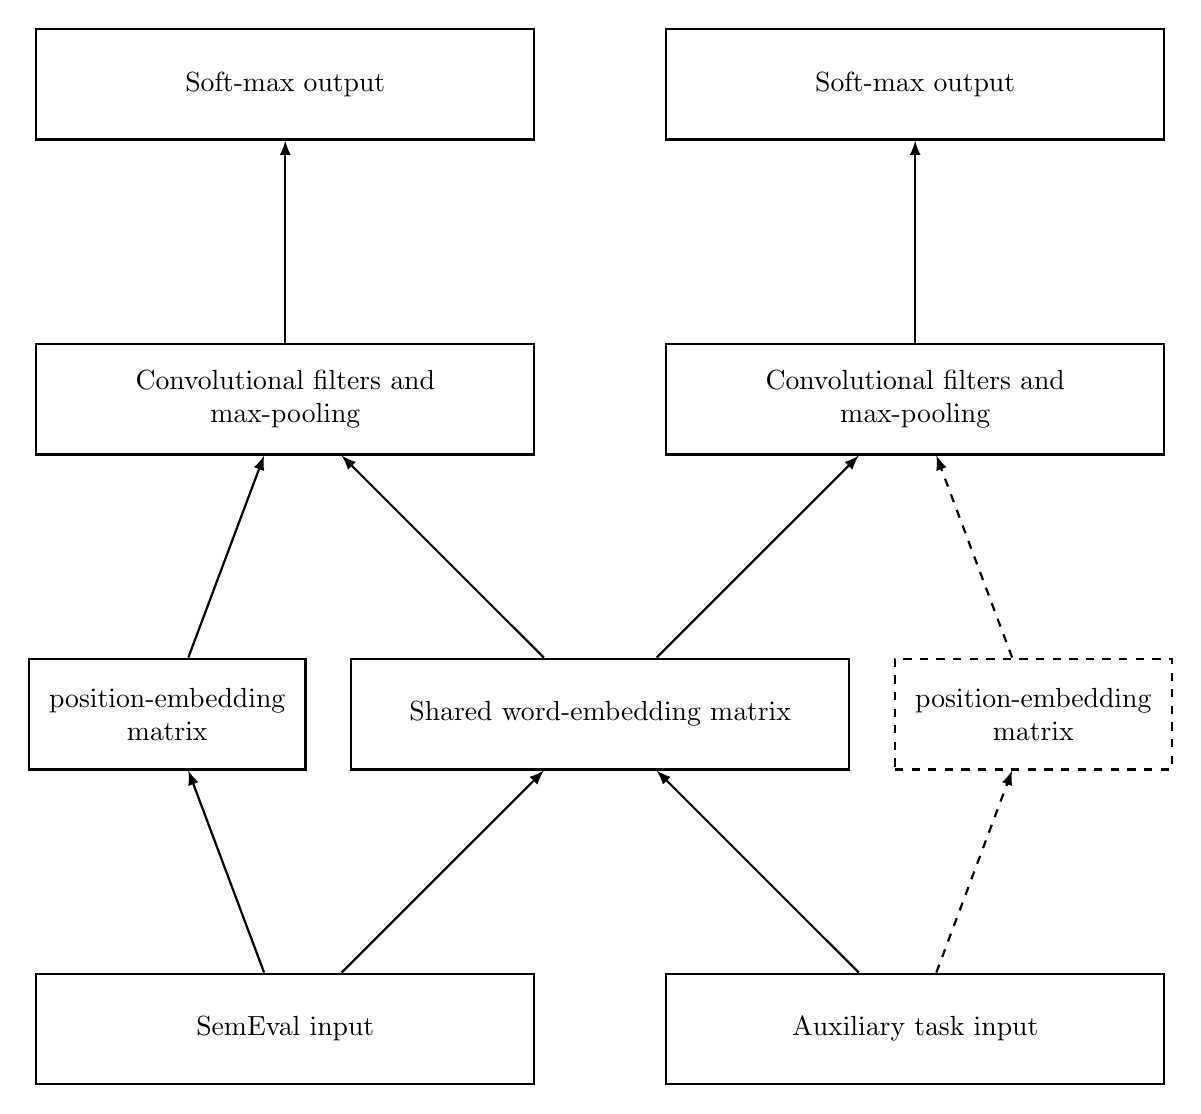
\begin{tikzpicture}
		\node [box] (embedding) at (0,0) {Shared word-embedding matrix};
		\node [draw=none,rectangle, align=center, minimum height=4em, draw, thick, minimum width=10em] (position_embedding) at (-5.5,0) {position-embedding\\matrix};
		\node [draw=none,rectangle, align=center, minimum height=4em, draw, thick, minimum width=10em, dashed] (position_embedding2) at (5.5,0) {position-embedding\\matrix};
		\node [box] (convolutions_task1) at (4,4) {Convolutional filters and\\max-pooling};
		\node [box] (convolutions_task2) at (-4,4) {Convolutional filters and\\max-pooling};
		\node [box] (output_1) at (4,8) {Soft-max output};
		\node [box] (output_2) at (-4,8) {Soft-max output};
		\node [box] (aux_sentence) at (4,-4) {Auxiliary task input};
		\node [box] (target_sentence) at (-4,-4) {SemEval input};
		\draw[-latex, thick] (target_sentence) edge (embedding);
		\draw[-latex, thick] (target_sentence) edge (position_embedding);
		\draw[-latex, thick] (aux_sentence) edge (embedding);
		\draw[-latex, thick] (embedding) edge (convolutions_task1);
		\draw[-latex, thick] (embedding) edge (convolutions_task2);
		\draw[-latex, thick] (convolutions_task1) edge (output_1);
		\draw[-latex, thick] (convolutions_task2) edge (output_2);
		\draw[-latex, thick] (position_embedding) edge (convolutions_task2);
		\draw[-latex, thick, dashed] (aux_sentence) edge (position_embedding2);
		\draw[-latex, thick, dashed] (position_embedding2) edge (convolutions_task1);
	\end{tikzpicture}
	\caption{Diagram of how neural network weights are shared between auxiliary tasks and SemEval 2010 Task 8. The word-embedding matrix is shared between tasks, but the convolution filters are not.}
	\label{relation_sequence_weight_sharing}
\end{figure}
\section{Algorithm}

Our main goal is to investigate the sample complexity dynamics of learning a relation classification task in a multi-task learning setting. To this end, we compare the generalisation error of a deep learning model trained only on SemEval 2010 Task 8, the target task, with the generalisation error of a deep learning model trained jointly on the SemEval data and one of the auxiliary tasks described in \ref{auxiliary_tasks}.
\\\\
We proceed as follows: We vary the amount of data from the target task and auxiliary task in turn by a set of fractions. For every combination of fractional target and auxiliary data, we perform 5-fold cross validation on the target data to yield 5 macro-F1 scores. We use the training data from the 4 training folds of target data and the auxiliary data to train the architecture described in \ref{network_architecture}. This is done by uniformly selecting one of the two tasks, sampling a mini-batch of the fractional training data from that task, and performing one gradient descent update with respect to cross-entropy error using the Adam algorithm described in section \ref{adam}. 
\\\\
This process is iterated until an early stopping criterion on the target training data is met. Specifically, $1/10$ of target training data is set aside for early stopping validation. When the cross-entropy error on the early stopping dataset has not improved for 200 iterations of mini-batch gradient descent, training is halted, and the model weights are reset to their best recorded value.

When the patience is exceeded we record the cross-validation macro-F1 on the target task test fold using the best recorded weights. Since neural network training is a random search procedure with respect to weight initialization and mini-batch sampling, we run this experiment for each combination of target and auxiliary fractional data 5 times, yielding a total of 25 random cross-validation splits for each combination. We have provided the algorithm used in our experiments as pseudocode in algorithm \ref{experiment_pseudocode}.
\begin{algorithm}
\begin{algorithmic}
	\Require $miniBatchSize$: an integer giving the mini-batch size
	\Require $targetData = \{(\vector{x}_{t1},\vector{y}_{t1}),\dots,(\vector{x}_{tN},\vector{y}_{tN})\}$
	\Require $auxiliaryData = \{(\vector{x}_{a1},\vector{y}_{a1}),\dots,(\vector{x}_{aN},\vector{y}_{aN})\}$
	\Require $sample(data, fraction)$: A routine that can sample $|set| \cdot fraction$ samples from the set $data$ uniformly.
	\Require $crossValidation(data)$: A routine that returns a set of cross-validation folds over the set $data$.
	\Require $initializeWeights()$: A routine that can initialize a neural network weight vector.
	\Require $gradientDescent(data, w)$: A routine that performs gradient descent on the neural network weights $w$.
	\Require $macroF1(w, data)$: A routine that computes the macro F1 score on $data$ using neural network weights $w$.
	\Require $report(score, targetFraction, auxiliaryFraction)$: A reporting routine.
	\State $fractions \gets \{\frac{0}{5}, \frac{1}{5}, \frac{2}{5}, \frac{3}{5}, \frac{4}{5}, 1\}$
	\For{$iteration \in \{1,\dots,5\}$}
		\For{$targetFraction \in fractions$}
			\For{$auxiliaryFraction \in fractions$}
				\State $targetFractionalData \gets sample(targetData, targetFraction)$
				\State $auxiliaryFractionalData \gets sample(auxiliaryData, auxiliaryFraction)$
				\State $earlyStoppingData \gets sample(targetFractionalData, \frac{1}{10})$
				\State $targetTrainData = targetFractionalData \setminus earlyStoppingData$
				\For{$trainFold, testFold \in crossValidation(targetTrainData)$}
					\State $\vector{w} \gets initializeWeights()$
					\While{\textit{patience not exceeded}}
						\State $task \gets sample(\{trainFold, auxiliaryFractionalData\}, \frac{1}{2})$
						\State $miniBatch \gets sample(task, \frac{|task|}{miniBatchSize})$
						\State $\vector{w} \gets gradientDescent(miniBatch, \vector{w})$
					\EndWhile
					\State $score = macroF1(\vector{w}, testFold)$
					\State $report(score, targetFraction, auxiliaryFraction)$
				\EndFor
			\EndFor
		\EndFor
	\EndFor
\end{algorithmic}
\caption{Pseudocode for our deep multi-task learning experiment.}\label{experiment_pseudocode}
\end{algorithm}
